\documentclass{standalone}
\begin{document}
	\subsection*{Multi Channel Image}
	
		This step involves the preparation of images, with the building of the multi channel image that incorporates neighbouring and edges information. 
		The used image is composed by 4 channel built as follows:  
		\begin{itemize}
			\item Pure image after Contrast Limited Adaptive Histogram Equalization (CLAHE), with a block size of  $10\times 10$ pixels
			\item Image after a median blurring with kernel size equal to $11$ pixes
			\item Image after a gamma correction with $\gamma = 1.5$
			\item Standard filtered image with a kernel of size $3$ pixels
		\end{itemize}
	
		\begin{figure}[h]
			\centering
				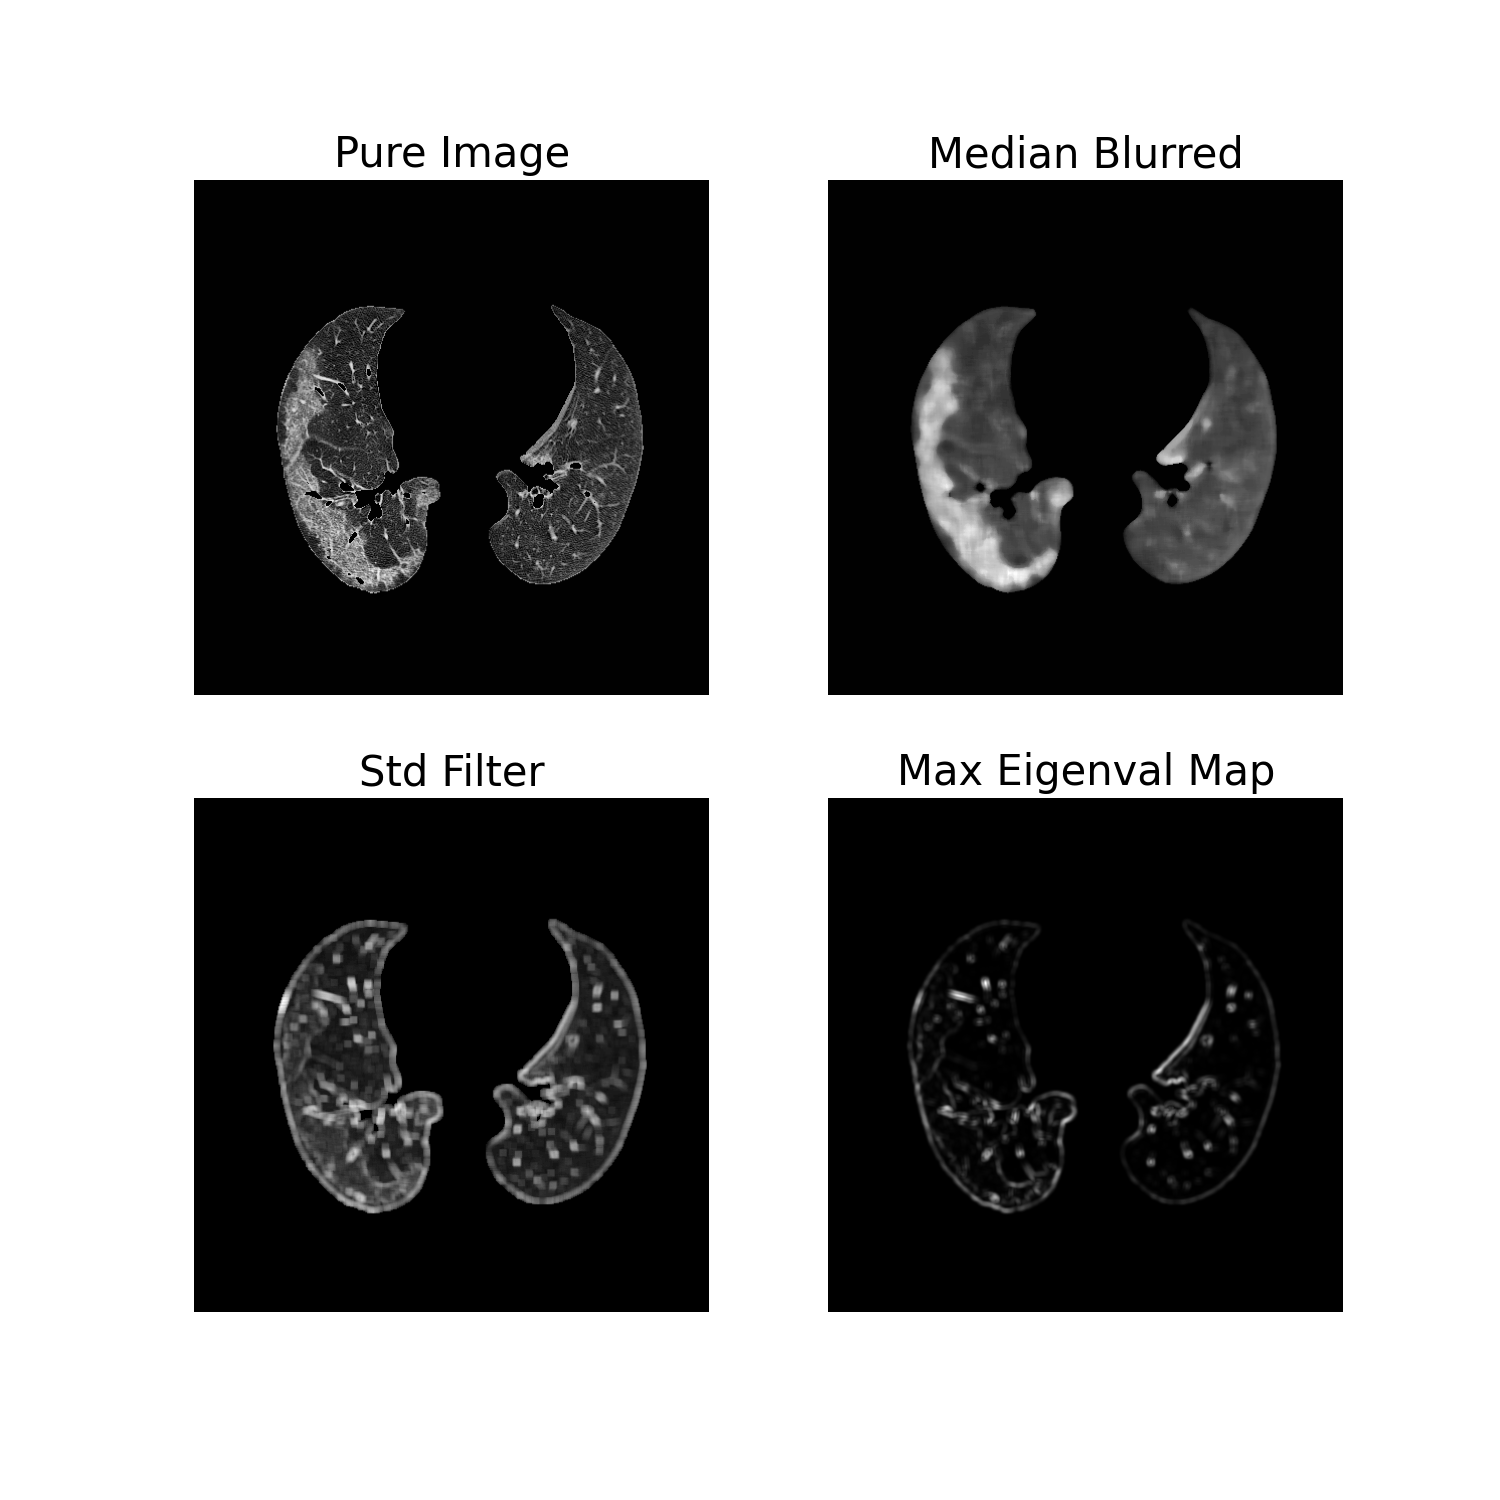
\includegraphics[scale=.55]{Multi_Channel.png}
			\caption{Channels of the image. From left to right and from top to bottom the image after the histogram equalization, the gamma correction, the median blurring and the std filtering. These channels allow us to consider information about single voxels, neighbouring voxels and their variability. The histogram eqaulization is applied over small $10\times 10$ areas to avoid  over-amplification of the contrast. The gamma correction was performed using $\gamma = 1.5$, and the median and std filter kernel sizes are respectively $11$ and $3$. Each image is normalized according to mean and standard deviation of the whole scan. }\label{fig:MultiChannel}
		\end{figure}
	
		In \figurename\,\ref{fig:MultiChannel} I have displayed the 4 different channels of the image. Each channel allow us to consider different information.
		
		The histogram equalized image and the gamma corrected allows to take into account information about the single voxel. The histogram equalization is applied in order to enhance the image contrast by improving the GL usage. For each slice the histogram is equalized considering only a $10\times 10$ area, in order to take care of the over-amplification of the contrast.
		
		The gamma correction is a non linear operation and is used to decode the luminance, and to made in evidence the less evident lesions. 
		
		The median blurring allow us to consider also the information of the neighborhood voxels, allowing the reduction of the outliers. The usage of the filter is justified since the lesions involves several closest voxels.
		
		The last channel cosist in the image after the application of a local standard deviation filter. This filter consist in the replacement of each pixel value with the standard deviation of its neighborhood. It help us to distinguish the bronchial structures and motion artifacts not removed during the lung segmentation.	
		
		Each image channel is normalized according to means and standard deviation of the whole scan; because of the k-means clustering.
\end{document}